\chapter{Network Security}
\section{History and Terminology}

\subsection{H/P/V/A/C}
\begin{itemize}
    \bullpara{Hacker}{
        \\ Highly competent computer ethusiast/engineer
        \begin{center}
            \begin{tabular}{l l}
                White Hat & Informs organisations of vulnerabilities before going public. \\
                Grey Hat  & Only informs if paid.                                         \\
                Black Hat & Malicious, uses findings to do illegal activity.              \\
            \end{tabular}
        \end{center}
    }
    \bullpara{Phreaker}{
        \\ Phone hacker, as phone network has become more digital they have been more often in the hacker category.
    }
    \bullpara{Virii}{
        \\ Computer virus creators.
        \begin{center}
            \begin{tabular}{l l}
                Ransomware & Encrypt files, decrypt for ransom.                                \\
                Spyware    & Keyloggers, browser addons to track, often include adware.        \\
                Trojans    & Software for botnet zombies, often appear as legitimate software. \\
            \end{tabular}
        \end{center}
    }
    \bullpara{Anarchist}{
        \\ Politically active hackers, when peaceful called hacktavists, when not so much they are anarchists. Some parts of the anonymous movement could be considered anarchists.
    }
    \bullpara{Crackers}{
        \\ Make use of tools built by others (e.g purchasing virus software, infiltration tools). Most modern digital organised crime would be in this category.
    }
    \bullpara{DDoSers}{
        \\ Someone who participates in \textbf{Distributed Denials of Service} attacks. \href{https://en.wikipedia.org/wiki/Low_Orbit_Ion_Cannon}{\textbf{Low Orbit Ion Cannon}} is an example, it is used to stress tests networks.
    }
    \bullpara{Spammers/Botters}{
        \\ Send unsolicited messages (often advertisements) en-masse, usually using botnets.
    }
    \bullpara{Warez}{
        \\ Information piracy, distribution software, images \& videos without the legal right to do so. Examples include the \href{https://en.wikipedia.org/wiki/The_Pirate_Bayhttps://en.wikipedia.org/wiki/The_Pirate_Bay}{priate bay} piracy site.
    }
    \bullpara{Whistleblowers}{
        \\ Former employees of an organisation that leak/"blow the whistle" on often malicious, illegal, or immoral activity even when it is illegal to do so (e.g have signed a \textbf{Non-Disclosure Agreement}).
    }
    \bullpara{Social Engineers}{
        \\ Use of social manipulation to compromise the human security of an organisation.
        \begin{center}
            \begin{tabular}{l l}
                Phising    & Usually over email, pretending to be some organisation they are not. \\
                Vishing    & Via voice messages.                                                  \\
                Smishing   & Via \textbf{SMS}.                                                    \\
                Catfishing & Via impersonation (e.g fake social media profiles).                  \\
            \end{tabular}
        \end{center}
    }
\end{itemize}

\subsection{Black Hat Methods}
\begin{itemize}
    \bullpara{Credential Reuse/Stuffing}{
        \\ Previously leaked login credentials are used against many sites (often people use the same email and password comnbination on many sites).
        \\
        \\ The site \href{https://haveibeenpwned.com/}{have I been pwned} can be used to check if your own details are included in any leaks.
    }
    \bullpara{Packet Sniffing}{
        \\ Monitoring network traffic not intended for your \textbf{NIC}, e.g over a wireless network, on a router or switch you control.
    }
    \bullpara{Code/SQL Injection}{
        \\ Using data infput to get a system to runb your code. If the system does not sanitise its input, some keywords or code contained may be executed. This is often SQL Injection, as most opportunities to input data are related to databases. An example is the log4j bug/exploit expained well by \href{https://www.youtube.com/watch?v=uyq8yxWO1ls}{this video}.
    }
    \bullpara{Session/Cookie Hijacking}{
        \\ Stealing a session cookie to be authenticated as them in an ongoing browser session.
    }
    \bullpara{Wardriving}{
        \\ Searchinbg for and abusing open/unsecure \textbf{WiFi}s.
    }
    \bullpara{Trashing/Dumpster Diving}{
        \\ Checking physical waste for useful informatrion (e.g bank statements, official records).
    }
    \bullpara{Clickjacking}{
        \\ Using hidden html divs, popups to force a user's click to redirect to a malicious destination.
    }
    \bullpara{Bait \& Switch}{
        \\ Luring a user to click with a seemingly legitimate advertisement, only to redirect them to something else.
    }
    \bullpara{Spoofing}{
        \\ Falsifying identification to receive packets intended for another recipient.
        \begin{center}
            \begin{tabular}{l l}
                IP  & Fake your IP as another (Layer 3).                                             \\
                MAC & Media Access Control address distinguishes between different \textbf{NICs}.    \\
                DNS & DNS cache poisoning (falsifying the cache to pretend to be at a given domain). \\
            \end{tabular}
        \end{center}
    }
    \bullpara{Rootkits}{
        \\ Allows attackers to secretly enter external systems, often installed as part of a virus.
    }
    \bullpara{Keyloggers}{
        \\ Records all keyboard input, sending key-logs back to the hacker, or allowing them to be remotely accessed.
        \\
        \\ A potential advantage of password managers is that keyloggers cannot be used effectively to detect passwords if they are not typed.
    }
    \bullpara{Trojans}{
        \\ Allow a hacker to remotely control an entire system, often as a zombie on a botnet.
    }
    \bullpara{Evil Twin}{
        \\ Where a hacker attempts to lure victims into using their network, gaining information from the victim (e.g network histroy) \& potentially sending malicious data to the user when they use it.
    }
\end{itemize}
\subsection{White Hat Tools}
\begin{itemize}
    \bullpara{Tails}{
        \\ \href{https://tails.boum.org/}{Tails} is a portable operating system designed to be usable from a usb drive, and to never store data, thus removing data integrity related security issues.
    }
    \bullpara{Kali Linux}{
        \\ \href{https://www.kali.org/}{Kali is} an operating system designed for penetration testing and other security related work. It comes bundled with many useful tools such as \textbf{Metasploit} and \textbf{Nmap}. It is supported on ARM, as well as by the windows subsystem for linux.
    }
    \bullpara{Metasploit}{
        \\ \href{https://www.metasploit.com/}{Metasploit} is a tool use to automatically scan systems for vulnerabilities based on a large database of known vulnerabilities and exploits.
    }
\end{itemize}

\subsection{Cybercrime Laws}
In the \textbf{UK} many laws (listed below) apply. Physical locations of hosts is used to determine which nation's laws are used, meaning \textbf{US} law is also very important (common country to host from).
\begin{center}
    \begin{tabular}{l l}
        1964 & \href{https://www.legislation.gov.uk/ukpga/1964/74/contents}{Obscene Publications Act} (In reference to spam)                                           \\
        1978 & \href{https://www.legislation.gov.uk/ukpga/1978/37/contents}{Protection of Children Act} (In reference to online abuse \& spam against children online) \\
        1988 & \href{https://www.legislation.gov.uk/ukpga/1988/48/contents}{Copyright, Designs and Patents Act}                                                        \\
        1990 & \href{https://www.legislation.gov.uk/ukpga/1990/18/contents}{Computer Misuse Act}                                                                       \\
        1999 & \href{https://www.legislation.gov.uk/ukpga/1999/14/contents}{Amendment to the Protection of Children Act} (Still being changed)                         \\
        2000 & \href{https://www.legislation.gov.uk/ukpga/2000/36/contents}{Freedom of Information Act}                                                                \\
        2000 & \href{https://www.legislation.gov.uk/ukpga/2000/23/contents}{Regulation of Investigatory Powers Act} (In reference to computer/phone surveillance)      \\
        2002 & \href{https://www.legislation.gov.uk/uksi/2002/2013/made}{e-Commerce Regulations Directive}                                                             \\
        2003 & \href{https://www.legislation.gov.uk/ukpga/2003/44/contents}{Criminal Justice Act}                                                                      \\
        2005 & \href{https://www.legislation.gov.uk/ukpga/2005/13/contents}{Disability Discrimination Act} (In reference to online abuse \& spam)                      \\
        2010 & \href{https://www.legislation.gov.uk/uksi/2010/2694/contents/made}{Amendment to the Copyright, Designs and Patents Act}                                 \\
        2013 & \href{https://www.legislation.gov.uk/ukpga/2013/26/contents}{Defamation Act} (In reference to online abuse \& spam)                                     \\
        2017 & \href{https://www.legislation.gov.uk/ukpga/2017/30/contents}{Digital Economy Act}                                                                       \\
        2018 & \href{https://www.legislation.gov.uk/ukpga/2018/12/contents}{Data Protection Act}                                                                       \\
    \end{tabular}
\end{center}
In the \textbf{US} there is the \href{https://www.copyright.gov/dmca/}{DMCA} (Digital Millennium Copyright Act).
\subsection{Standards Organisations}
\begin{center}
    \begin{tabular}{l p{0.8\textwidth}}
        \href{https://www.iana.org/}{IANA}            & Internet Assigned Numbers Authority, deals with \textbf{DNS}, \textbf{IP} Addressing and more standards.                                                               \\
        \href{https://www.icann.org/}{ICANN}          & A nonprofit organisations responsible for coordinating standards for the maintenance and running of namespace and numerical space databases for the internet.          \\
        \href{https://www.ietf.org/}{IEFT}            & Internet Engineering Task Force, a collection of working groups (e.g routing, transport, security) concerned with developing the internet.                             \\
        \href{https://www.internetsociety.org/}{ISOC} & Internet Society, dedicated to furthering beneficial use of the internet.                                                                                              \\
        \href{https://www.eff.org/}{EFF}              & Electronic Frontier Foundation, a politically active nonprofit dedicated to defending privacy, free speech and freedom to innovate online.                             \\
        \href{https://www.w3.org/standards/}{W3C}     & The World Wide Web Consortium develops standards to help developers build tools on the web smoothly.                                                                   \\
        \href{https://www.iso.org/}{ISO}              & International Organisation for Standardization, you can find their standards for information technology \href{https://www.iso.org/committee/45020/x/catalogue/}{here}. \\
    \end{tabular}
\end{center}
\subsection{Attack Examples}

\begin{definitionbox}{Heartbleed}
    A bug in OpenSSL 1.0.1 first identified onm 14/03/2012 and patched on 07/04/2014.
    \\
    \\ OpenSSL is an implementation of the TLS (transport Layer Security)/SSL (Secure Sockets Layer) protocol that allows for secure website access (\lstinline{https://})
    \\
    \\ The bug allowed users to gradually reveal server memory in chunks of $64KB$. It is not known if it was used in any exploits.
\end{definitionbox}
\begin{definitionbox}{KRACK}
    The \textbf{WPA2} (wireless protected access protocol) used in Wifi. Android devices could be forced to use a zero-based key, rendering the encryption useless.
    \\
    \\ The full explanation can be found \href{https://www.krackattacks.com/}{here}.
    \\
    \\ It has been patched, but the next version (\textbf{WPA3}) was released in 2020 which was meant to be more secure also has issues.
\end{definitionbox}
\begin{definitionbox}{WEP}
    \textbf{Wired Equivalent Privacy} is a security algorithm for wireless networks, it has been shown to be vulnerable many times.
\end{definitionbox}

\section{Network Security Issues}
\subsection{Basic Security Concepts}
\begin{center}
    \begin{tabular}{l p{0.8\textwidth}}
        Access Control  & Only certain users can access certain resources.                                                                 \\
        Authentication  & User knows resource is as identified, and resource that user is as identified.                                   \\
        Confidentiality & Users can limit access to their resources and information, and limit access to see their traffic over a channel. \\
        Data Integrity  & Users cannot damage the integrity of a resource (e.g crash a webserver by visiting).                             \\
        Non-Repudiation & User cannot deny communication occurred, secure logs held and can be audited.                                    \\
    \end{tabular}
\end{center}

\subsection{Access Control}
\begin{center}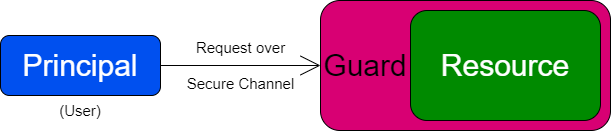
\includegraphics[width=0.6\textwidth]{network_security/images/access control.png}\end{center}
Assuming the channel used for communication is secure, the guard needs to determine:
\begin{itemize}
    \setlength\itemsep{0em}
    \item Which principals (users) can access the resource.
    \item Where principals can be located (e.g user's \textbf{IP} address is outside the organisation's network).
    \item What requests principals can make for this resource (e.g can view database, but not send mutating \textbf{SQL} commands).
\end{itemize}
Security can be difficult as:
\begin{itemize}
    \setlength\itemsep{0em}
    \item Many systems used by an organisation can be different (Heterogeneous systems) (e.g bank has different OSes several models of ATM).
    \item Users can be careless (e.g reusing passwords), this include system administrators and managers.
\end{itemize}
\subsection{Firewalls}
\begin{definitionbox}{Firewall}
    A security barrier between internal and external networks.
    \begin{itemize}
        \setlength\itemsep{0em}
        \bullpara{Application Level Gateway}{
            \\ An application that runs, checks requests in the application layer. Can also be a proxy, using an extra set of rules to decide if to share requests or responses, or to send on requests.
            \\
            \\ Examples include \textbf{SOCKS} and \href{https://www.netfilter.org/projects/iptables/index.html}{netfilter's iptables}.
        }
        \bullpara{Proxy Server}{
            \\ Runs on the network protecting it by making requests and receiving responses on its behalf (to the external network). Can also include caching of results.
        }
        \bullpara{Circuit Level Gateway}{
            \\ Creates a circuit of proxies, sending data between each node in the circuit (for example \textbf{Tor}).
        }
        \bullpara{Packet Filtering}{
            \\ Filtering packets with a set of rules based on contents, source and destination IP address/port, only alowing non-suspect packets through. Can also be stateful, considering not just a single packet traffic to a host over some time period.
        }
        \bullpara{Hybrid}{
            \\ Use a combination of all the above.
        }
    \end{itemize}
    They can be software or hardware based, with hardware solutions being faster, but more difficult to change (e.g if a vulnerability is found).
\end{definitionbox}

\begin{definitionbox}{Proxy}
    Makes requests and recieved responses on behalf of a client, can filter in and outgoing traffic.
    \begin{itemize}
        \setlength\itemsep{0em}
        \bullpara{Normal}{ \\ Client is aware of proxy, and connects to it to use it.}
        \bullpara{Transparent}{ \\ Client is unaware, for example a local router could act as a proxy. Requires not intervention from client.}
        \bullpara{Reverse}{ \\ Runs on the receiving side, impersonating a server and protecting a server from the external network. (Much like \textbf{CDN} load balancing) }
    \end{itemize}
\end{definitionbox}
\begin{definitionbox}{Bastion Host}
    A server that expects to be attacked.
    \begin{itemize}
        \setlength\itemsep{0em}
        \item Runs a minimal trusted/secure OS.
        \item Only essential applications (e.g no window manager needed).
        \item All possible limits enabled (readonly file system, no mounts, file permissions all set, no normal user accounts)
        \item Typically managed over a dedicated terminal
    \end{itemize}
    It passes requests on from the external network, and acts as a proxy firewall.
    \\
    \\ It drops any connections it determines are suspect using packet filtering (usually stateful) and other techniques.
\end{definitionbox}
\begin{examplebox}{iptables}
    \fun{iptables} can be used on linux to set packet filters. It consists of several tables, each containing chains of rules on managing network packets.
    \\
    \\ Note that it requires root as it interfaces directly with the linux kernel's firewall.
\end{examplebox}
\begin{examplebox}{tcpd}
    The linux \textbf{TCP} Daemon controls access to unix services \& can monitor requests to services (e.g \fun{ftp}, \fun{exec}, \fun{rsh}, \fun{telnet}).
    \\
    \\ It uses two files, \lstinline{/etc/hosts.allow} and \lstinline{/etc/hosts.deny} to determine access.
\end{examplebox}

\subsection{Firewall Avoidance}
\subsubsection{SSH}
We can attempt to avoid a firewall by tunneling through with an allowed protocol, to then use the internal.
\\
\\ An example of this is with \textbf{ssh}. We can get through the firewall on ssh, and then send our requests through ssh to the internal network, to get responses, and use services the firewall may normally block.

\subsubsection{Spoof MAC Address}
Can re-write the \textbf{MAC} address if the firewall is blocking requests based on it (MAC address blacklisting or whitelisting).

\subsubsection{Spoof IP Address}
Much like with \textbf{MAC} address, however stateful firewalls will most likely detect this.

\subsubsection{(VPN) Virtual Private Network}
Much like with \textbf{SSH}, we can tunnel through the firewall. Provided the tunnel is secure (e.g using \textbf{SSL}) the firewall will not be able to decipher your traffic.

\subsection{Other Security}
\begin{definitionbox}{(IDS) Intrustion Detection System}
    Detects intrustions to inform the system (e.g a DDoS attack), however does not perform actions to stop the detected intrusion.
\end{definitionbox}
\begin{definitionbox}{(IPS) Intrusion Prevention System}
    Actively prevents intrusions (e.g blocking \const{SYN} flooders attempting to perform a DDoS attack), can work with an \textbf{IDS}.
\end{definitionbox}
\begin{definitionbox}{(NGFW) Next Generation Firewall}
    A stateful firewall that comes with an \textbf{IPS} / \textbf{IDS} system.
\end{definitionbox}
\begin{definitionbox}{(UTM) Unified Threat Management}
    Similar to a \textbf{NGFW} but with added features such as spam filters, antivirus etc.
\end{definitionbox}
\subsection{(DMZ) Demilitarized Zone}
\begin{center}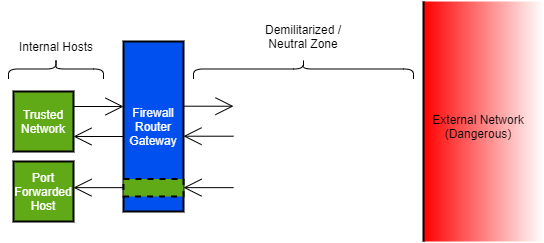
\includegraphics[width=0.7\textwidth]{network_security/images/DMZ.png}\end{center}
\begin{definitionbox}{(NAT) Network Address Translation}
    Rather than expose the \textbf{LAN} \textbf{IP} address of an internal host, routers translate the IP addresses to their own public IP to send, and when receiving from their public IP back to the IPs of internal hosts.
\end{definitionbox}
\begin{definitionbox}{Port Forwarding}
    To expose an internal host to the external network without placing it in the \textbf{DMZ} we can set the router to forward all packets arriving at a given port straight to the internal host.
    \\
    \\ For example we could specify any packet recieved on the router's IP at port $3472$ should be immediately forwarded to the \textbf{NAT} based \textbf{LAN} \textbf{IP} of "host A" on port 80.
    \\
    \\ Useful for hosting servers, even for games (e.g minecraft servers require port forwarding).
\end{definitionbox}
\subsection{Logging and Auditing}
Most systems keep logs, they are useful for:
\begin{itemize}
    \setlength\itemsep{0em}
    \item Checking for missed breaches. An attack may only be discovered in logs after the fact.
    \item Forensics, providing evidence to law enforcement to discover who the purputrators of an attack are.
    \item Determining how a system was exploited in an attack, in order to patch it.
    \item Ensuring good practices are being followed (e.g if an unsafe features starts to be used).
    \item Detecting other network issues (e.g congestion).
\end{itemize}
Logs can be found on linux at \lstinline{/var/log/} and the event viewer in Windows.

\section{Cryptography}
\begin{center}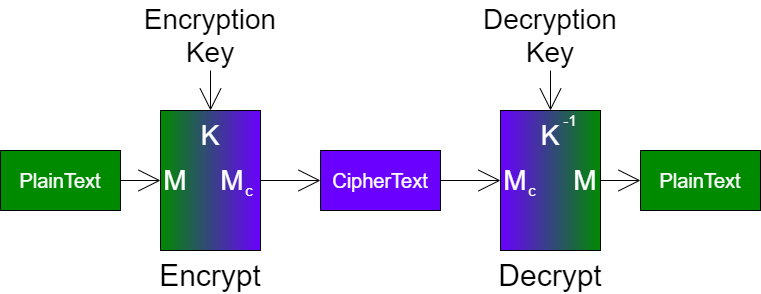
\includegraphics[width=0.9\textwidth]{network_security/images/cryptography.png}\end{center}
A good encryption algorithm should ensure:
\begin{itemize}
    \setlength\itemsep{0em}
    \item Given $M_C$ it is only possible to find $M$ by going though all possible values of $K^{-1}$ (brute force attack).
    \item Given $M$ and $M_C$ it should be difficult to get the values of $K$ and $K^{-1}$. (e.g caesar cipher is poor as we can just calculate the shift)
\end{itemize}
\begin{definitionbox}{Symmetric and Secret Key Encryption}
    \begin{center}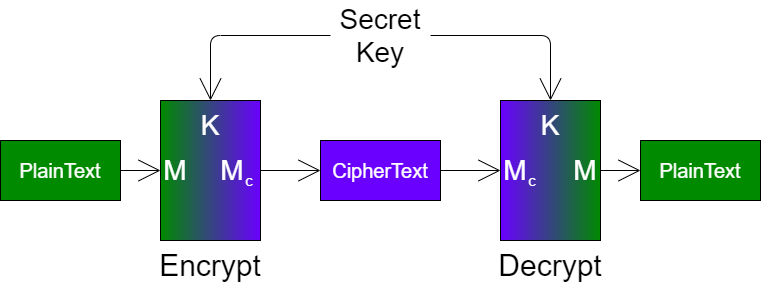
\includegraphics[width=0.9\textwidth]{network_security/images/cryptography symmetric.png}\end{center}
    The same key is used for encryption and decryption (symmetric), and this key is secretly shared between sender and receiver (not on an unsecure channel) (secret).
    \begin{itemize}
        \setlength\itemsep{0em}
        \item Must secretly disclose key to communicate.
        \item Faster encryption/decryption than \textbf{Asymmetric}.
    \end{itemize}
    An example is \textbf{DES} (\textbf{Data Encryption Standard}), though this has a short key length and is now too insecure for general use (wikipedia article \href{https://en.wikipedia.org/wiki/Data_Encryption_Standard}{here}).
\end{definitionbox}
\begin{definitionbox}{Asymmetric and Public Key Encryption}
    Each user has a \textbf{public} and \textbf{private} key.
    \\
    \\ For confidentiality: Sender encrypts with receiver's public, receiver decrypts with their private.
    \begin{center}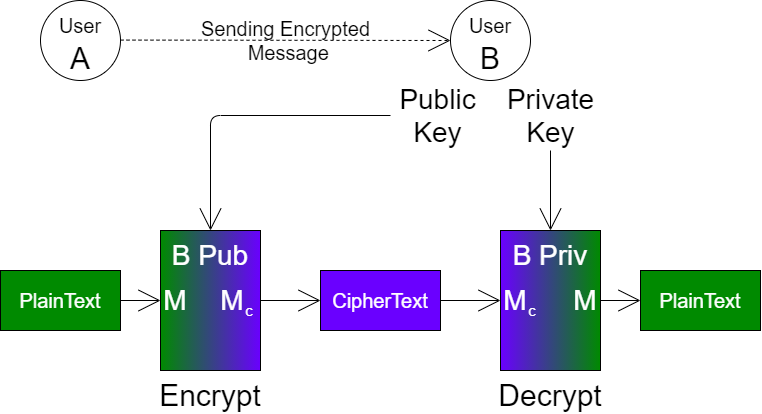
\includegraphics[width=0.9\textwidth]{network_security/images/cryptography asymmetric confidential.png}\end{center}
    For signing: Sender encrypts with their private key, receiver decrypts with sender's public key, if value was successfully decrypted then we know the message was from the sender with the public key we used.
    \begin{center}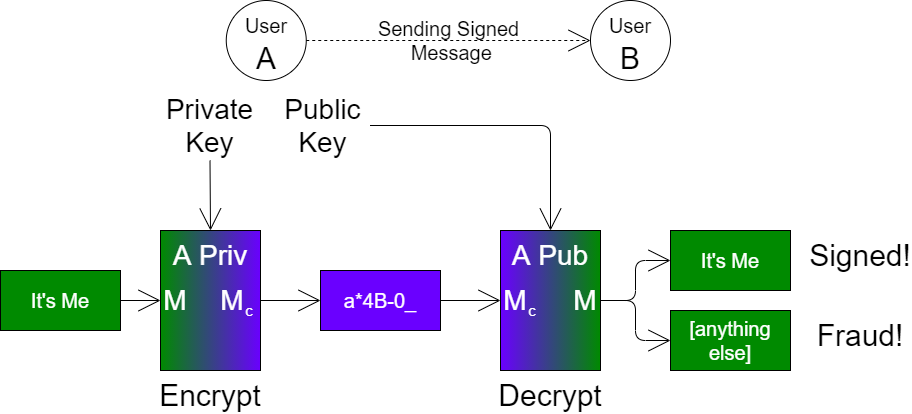
\includegraphics[width=0.9\textwidth]{network_security/images/cryptography asymmetric sign.png}\end{center}
    We can then combine these, encrypting a message, but including a signed segment inside to verify the sender. We can also combine with symmetric encryption to sign symmetrically encrypted files (e.g check if a password protected file is from the correct sender/is not tampered with). Foe example \href{https://gnupg.org/}{GPG}.
    \\
    \\ The main points are:
    \begin{itemize}
        \setlength\itemsep{0em}
        \item No need to disclose private information to communicate securely so, can start communication on unsecure channel.
        \item Hence more secure than \textbf{Secret Key} encryption.
        \item However is slower to encrypt and decrypt.
    \end{itemize}
    An example of this is \textbf{RSA} which uses current difficulty in prime factor decomposition to ensure brute force attacks are computationally intractable (wikipedia article is \href{https://en.wikipedia.org/wiki/RSA_(cryptosystem)}{here}).
\end{definitionbox}
\begin{definitionbox}{Diffie-Hellman Key Exchange}
    \begin{center}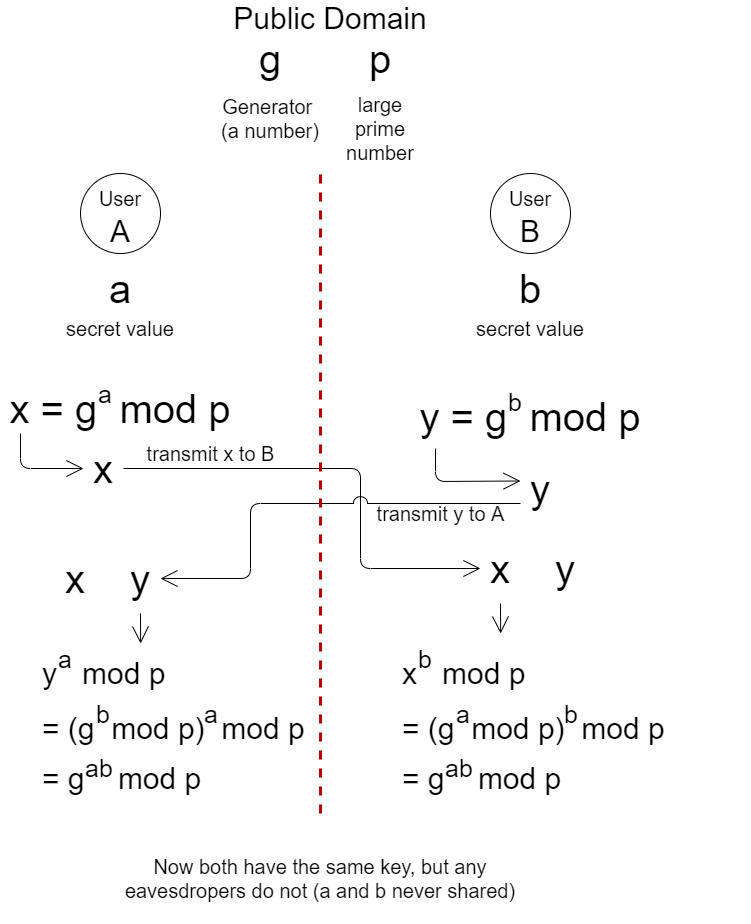
\includegraphics[width=0.9\textwidth]{network_security/images/diffie hellman key exchange.png}\end{center}
\end{definitionbox}
\begin{definitionbox}{Kerberos (Needham \& Schroeder)}
    A key distribution system for secret keys, using a trusted server.
    \begin{itemize}
        \setlength\itemsep{0em}
        \item Kerberos authenticates you with a password.
        \item It can also authenticate the user/resource you intend to communicate with.
        \item Generates a ticket which allows for communication.
        \item Ticket can be used up to a time limit, after which you must get another ticket.
        \item Originally vulnerable to \textbf{Man/Monster in the Middle} attacks, though these have since been addressed.
    \end{itemize}
\end{definitionbox}
\begin{definitionbox}{Hashing}
    In cryptography, a hash function converts some data into a fixed size alphanumeric string.
    \begin{itemize}
        \setlength\itemsep{0em}
        \item The same input data always produces the same hash value.
        \item Not possible to derive the original input from the hash value (unlike encryption).
        \item Can be used as a checksum to verify data (e.g that the contents of a file are unchanged/not tampered with).
        \item Many old hash functions have been broken (either algorithm issues, or all possible hashes now determines - rainbow tables).
    \end{itemize}
\end{definitionbox}

\section{WireShark}
\termdef{Credential Resuse/Stuffing}{
    Using previously leaked/found eail-passoword combinations on other services. Useful when users reuse passwords for mutliple services.
}
\termdef{Network Monitoring / Packet Sniffing}{
    Listening on a network and reading packets where you (your \keyword{NIC}) are not the intended recipient.
}
\termdef{Code/SQL Injection}{
    Executing code on a system by passing it through normal data collection.
    \\
    \\ e.g if text entered in a website is directly substituted into a database query, by writing SQL ocde in the text entry, we can alter (or add another query) to the query generated.
}
\termdef{Session/Cookie Hijacking}{
    Using the cookie/authentication token form another user's session to get authenticated.
}
\termdef{Wardriving}{
    Identifying and compomising unsecured wireless networks.
    \\
    \\ e.g installing spyware on usecured home routers.
}
\termdef{Wireshark}{
    Wireshark is a network protocol analyser. It allows users to capture, analyse \& deconstruct packets to analyse traffic on a network.
}
\subsection*{WireShark Modes}
\twosplit{
    \centerline{\keyword{Promiscuous Mode}}
    \compitem{
        \item Works for Wired and wireless.
        \item \keyword{NIC} does not drop packets, retains all received packets.
        \item When wireless, only listens on the connected network.
        \item Some \keyword{NIC}s ignore this (considered \textit{impolite} and easily abused).
    }
}{
    \centerline{\keyword{Monitor Mode}}
    \compitem{
        \item Only works on wireless networks.
        \item \keyword{NIC} listens on all networks in range/that it can receive from.
        \item Wifi networks secured with authentication (e.g password) will appear scrambled (encryption).
        \item Most \keyword{NICs} do not support this, may require new drivers or a special \keyword{NIC}.
        \item \keyword{WinPcap} (windows) does not support though \keyword{AirPcap} and \keyword{Npcap} on linux do.
    }
}

\sidenote{Sniffing Ethics}{
    When monitoring a network, it needs to be a netywork you have permission to monitor (either wired or wireless)
}
\subsection*{WireShark Packet Capture}
\begin{center}
    \begin{tabular}{l p{0.7\textwidth}}
        \textbf{Location} & \textbf{Can Capture}                                                                                                                    \\
        \hline
        \textbf{Hub}      & Local traffic, Broadcast/Multicast, (Promiscuous Mode) Entire Network.                                                                  \\
        \textbf{Switch}   & Local Traffic, Broadcast/Multicast, (Promiscuous Mode) Network connected to the same switch port.                                       \\
        \textbf{WLAN}     & Local Traffic, Broadcast/Multicast, (Promiscuous Mode) Entire WLAN, (Monitor Mode) All wireless packets physically receivable/in range. \\
    \end{tabular}
\end{center}
We can provide wireshark with authentication to allow it to decrypt packets on for protected networks (e.g provide the RSA key for SSL, or password for WPA/WEP).

\subsection{WireShark Display Filters}
Can hide or select packets based on contents, destination \& source address and more. And can build up complex filters.
\example{WireShark Capture Filter}{
    \codelist{Python}{network_security/code/wireshark_filter.py}
    \href{https://wiki.wireshark.org/DisplayFilters\#examples}{More Examples} and \href{https://www.wireshark.org/docs/wsug_html_chunked/ChWorkBuildDisplayFilterSection.html}{filter building tutorial}.
}

\subsection{NMAP}
\termdef{NMAP}{
    A network scanning tool which uses sends raw \keyword{IP} packets and monitors responses \& determine the services provided by the network and its hosts.
    \\
    \\ It can be used to detect vulnerable hosts on a network.
}
We can scan networks using the gui, or by using the command line utility:
\codelist{Bash}{network_security/code/nmap_examples.sh}